\documentclass[border=0pt]{standalone}
\usepackage{fontspec}
\setmainfont{Carlito}
\usepackage{unicode-math}
\setmathfont{Latin Modern Math}
\usepackage{xcolor}
\usepackage{booktabs}
\usepackage{tikz}
\usepackage{graphicx}

\definecolor{canvabg}{RGB}{246,244,241}
\definecolor{textDark}{RGB}{40,40,40}
\definecolor{textMute}{RGB}{125,120,113}
\definecolor{accent}{RGB}{18,125,108}
\definecolor{trough}{RGB}{160,55,50}
\definecolor{bridge}{RGB}{30,90,140}

\pagecolor{canvabg}

\providecommand{\Cref}[1]{}
\providecommand{\cref}[1]{}
\providecommand{\ab}[1]{#1}

\renewcommand{\arraystretch}{1.3}

\begin{document}
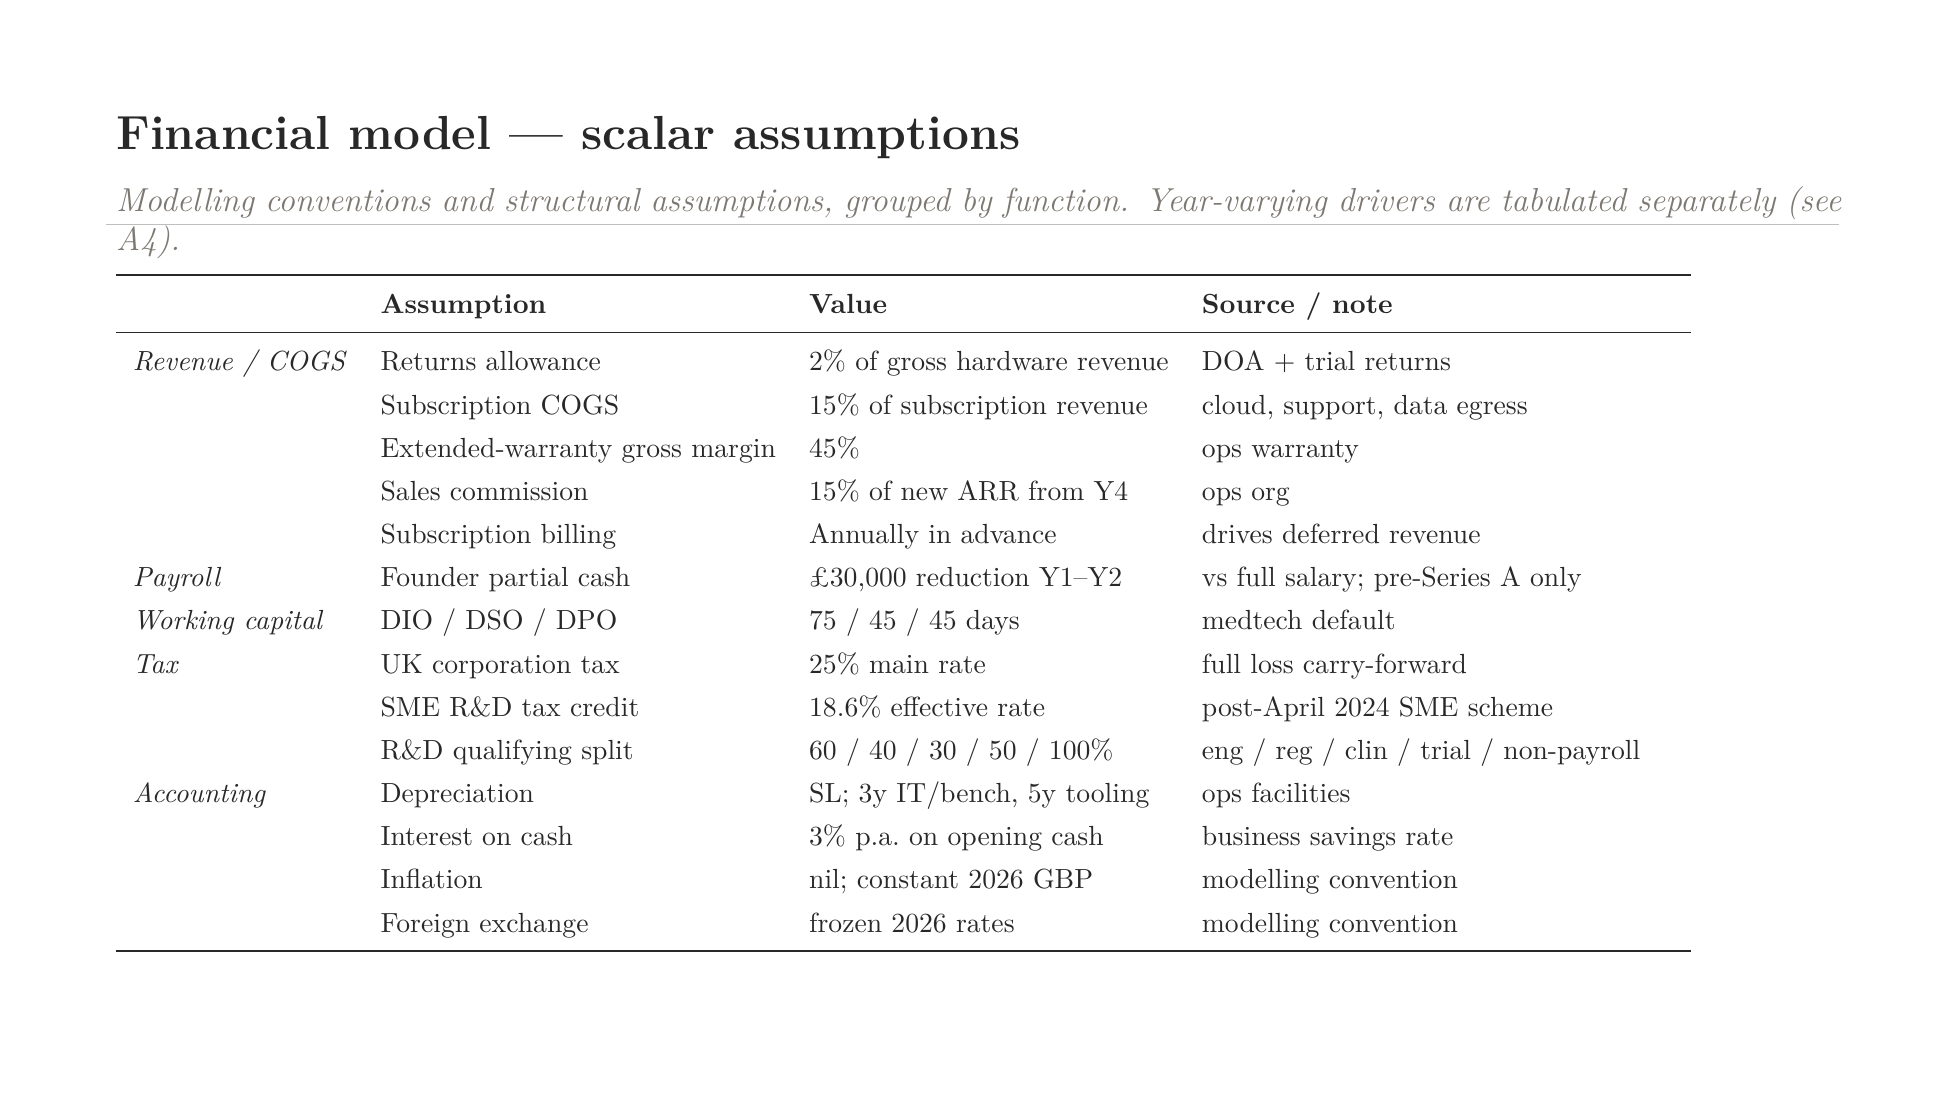
\begin{tikzpicture}[every node/.style={text=textDark}]
\useasboundingbox (0,0) rectangle (24, 13.5);

\node[anchor=north west, font=\bfseries\LARGE] at (1.0, 12.5)
    {Financial model — scalar assumptions};
\node[anchor=north west, font=\itshape\large, text=textMute, text width=22cm]
    at (1.0, 11.6)
    {Modelling conventions and structural assumptions, grouped by function.
     Year-varying drivers are tabulated separately (see A4).};

\draw[gray!50, line width=0.5pt] (1.0, 11.0) -- (23.0, 11.0);

\node[anchor=north west, font=\normalsize] at (1.0, 10.5) {%
\begin{tabular}{lllp{6cm}}
    \toprule
     & \textbf{Assumption} & \textbf{Value} & \textbf{Source / note} \\
    \midrule
    \textit{Revenue / COGS} & Returns allowance              & 2\% of gross hardware revenue   & DOA + trial returns \\
                              & Subscription COGS              & 15\% of subscription revenue    & cloud, support, data egress \\
                              & Extended-warranty gross margin & 45\%                            & ops warranty \\
                              & Sales commission               & 15\% of new ARR from Y4         & ops org \\
                              & Subscription billing           & Annually in advance             & drives deferred revenue \\
    \textit{Payroll}        & Founder partial cash           & \pounds 30{,}000 reduction Y1--Y2 & vs full salary; pre-Series A only \\
    \textit{Working capital} & DIO / DSO / DPO                & 75 / 45 / 45 days               & medtech default \\
    \textit{Tax}            & UK corporation tax             & 25\% main rate                  & full loss carry-forward \\
                              & SME R\&D tax credit            & 18.6\% effective rate           & post-April 2024 SME scheme \\
                              & R\&D qualifying split          & 60 / 40 / 30 / 50 / 100\%       & eng / reg / clin / trial / non-payroll \\
    \textit{Accounting}     & Depreciation                   & SL; 3y IT/bench, 5y tooling     & ops facilities \\
                              & Interest on cash               & 3\% p.a.\ on opening cash       & business savings rate \\
                              & Inflation                      & nil; constant 2026 GBP          & modelling convention \\
                              & Foreign exchange               & frozen 2026 rates               & modelling convention \\
    \bottomrule
\end{tabular}
};

\end{tikzpicture}
\end{document}
